% LINGI2255 - Software Development Project
% Phase 2 - Architecture report
% Framework choice
\documentclass[11pt, a4paper]{article}   	% use "amsart" instead of "article" for AMSLaTeX format
\usepackage[utf8]{inputenc}
\usepackage[UKenglish]{babel}
\usepackage{graphicx}

\usepackage{amssymb}
\usepackage{xcolor}
\usepackage{hyperref}
\usepackage{url}
\usepackage{csquotes}

\newcommand{\tbf}[1]{\textbf{#1}}
\newcommand{\tit}[1]{\textit{#1}}


\title{Brief Article}
\author{The Author}
%\date{}							% Activate to display a given date or no date

\begin{document}
%\maketitle

\section{Simulator}

We chose Selenium\footnote{\url{http://www.seleniumhq.org/}} to automate the testing of the web application.
An interesting feature is that we can actually see the actions performed in real time.

Selenium is composed of different components, but the one that we're interested in is the Selenium WebDriver\footnote{\url{http://www.seleniumhq.org/projects/webdriver/}}. % with the Selenium-Server
Its purpose is to drive a browser natively, either on a local or remote machine.
It gives the ability to send commands to a browser and to retrieve the results.
The Selenium WebDriver uses specific drivers to interact with browsers.
There are drivers for multiple browsers, including Chrome, Firefox and the Android browser.

\medskip
The tests can be written in multiple languages, including Java, Python and Ruby.
We chose to use Python because it is a simple, yet powerful language, and we will also use it for the web application.

\medskip
The simulator will not be integrated with the rest of the web application, because they are made for different purposes.
It will be useful to stress our system and to see how it adapts to such situations.
It will give us an idea of how the system performs in real conditions.


\section{Extension}

Our extension is social media.
It consists of allowing the users to login with a Facebook or Google account.
We decided to add the possibility to sign in with a Twitter account, because we think it could allow more users to easily use the web application.

\medskip
We will use the Django framework to build the web application, and it offers a built-in user authentication system.
It handles user accounts, groups, permissions and cookie-based user sessions. 
There are many packages available that can be installed to extend the possibilities of a Django project.
We searched for one that could help us for this task, and we chose to use the Django-Allauth\footnote{\url{https://www.djangopackages.com/packages/p/django-allauth/}} package to manage users authentication with Facebook, Google, or Twitter.
It is an interesting package because it supports a lot of authentication services, so that we could add more in the future if it is relevant.
Furthermore, it supports Python3 and Django 1.7, the latests stable versions.

\subsection*{How it will integrate with the system}
When the user sign in via a third-party provider, the module will create a \textit{user} object in the system as a standard registration.
The only difference is that this user will have no password associated.
Instead, another object \textit{Social account} will exists which will permit the user to sign in.
Since it is hard to automate registration and connection by third-party providers, we will not be able to test this extension via the simulator.


\section{User-Interface design}
The user interface has become increasingly important and complex.
Nowadays, UI frameworks are highly used by front-end developers.
Naturally, we looked for a UI framework that meets our needs.
\textit{Twitter Bootstrap} is a reference in this domain.
It encourage the use of responsive design, which means that the UI will adapt to the screen it is displayed on.
Furthermore, it promotes minimalist UI design that makes it is easier and quicker for the user to access information.


\section{Sequence diagrams}

For the sequence diagrams we picked the same use cases than the activity diagrams because in our first report it lacked some details.
In the second report, we added the create account sequence diagram because it is a important part of the software and it was missing from our first report.

In this report, we have modified some of the sequence diagrams taking into account the remarks made after our second report.

%\figure{requestingHelp}

On figure {requestingHelp} : The user need some help and he is going to create a new request. For that he click on the \enquote{I need help}
and he is redirected to a page where he needs to fill in informations about the jobs. Afterward the system check the data entered by the user.
If it is correct create the request and add it to the list of request on the home page. The system also send a notification to the members that
correspond to the criterias of the request using their preferences. If the data are not correct it send an error message to the user.

The main modification on figure {requestingHelp} is that the action \enquote{publish on home page} is now done by the system. You can see below the modified 
diagrams and their descriptions.

%\figure{completeAJob}

On figure {completeAJob} : The user has completed a job and want to get time credit for it. For that he needs to go to the pending actions page (list all the jobs that the member accepted but did not completed yet) and select the corresponding job. He will then fill informations about the job and confirm. 

The system will send a notification to the demanding member (member which has been helped) and this member need to confirm that the job has been done correctly.

Unfortunatly it can happen that the member does not confirm because for example, he has no internet access. In this case, after some times, the system will send a message to the branch officer and ask him to confirm by himself.

The main modification on figure {completeAJob} is that the system send a message to the branch officer if the demanding member does not confirm after a certain period of time. (I didn't find a way to show the waiting time)

\subsection{Login with Social Media}

In this report, we also added a new sequence diagram called \enquote{LoginWithSocialMedia}. We did that becaus in the second report we talked about the social media extension but we did not explain how we will integrate it in our own software.

%\figure{LoginWithSocialMedia}

On the figure {LoginWithSocialMedia} you can see that the client wants to authenticate using a social media like Google+ or Facebook. These social medias all give the possibility to sign in on your web site using their account. Usually they have multiple way to do it but the most common one is throw javascript using a API. We choose that approach because we plan to support multiple social media.

In fact in this diagram the client directly use javascript to contact the social media API server to login. Than the social media API server check first if the credential are correct and second if the user already allowed this website to access his account and ask the user permission otherwise. 
Finally the server send back the token which will be use to authenticate the user for the API calls and the client will send some informations about his account to our application.

\section{Deployment diagram}

In the second report, our explanation was a bit too technical here is the main reason without all the technical details.

We choosed Nginx because it is a very light and efficient web server. We use it as a reverse proxy to avoid putting too much load on our application server (Gunicorn). The Gunicorn workers are like multiple application server which will handle the work. We didn't use another web server for exemple apache because Nginx is faster and better for the usage we want to do with our web server.

\section{Class diagrams}

For the class diagram there was a few mistakes and some missing features about the social media extension. 

We tried to correct this by modifying our main class diagram and creating new small diagrams.


\subsection{Main class diagram}

%\figure{newMainClassDiagram}

On the figure {newMainClassDiagram} you can see some new things.

In our main class diagram we did the following changes :

\begin{itemize}
\item We added all the missing parameters to the function
\item We added new function to some classes 
\item We added type to attributes
\item We created new classes 
\end{itemize}

\subsubsection{class member}

The class member has now more functions :
\begin{itemize}
\item A function to share on a social Media like Facebook / Google+
\item Some functions to add/remove a user to/from their personnal network/favorite/ignored list.
\item Some functions to (un)subscribe to a branch.
\end{itemize}

\subsubsection{class help}

The class help has now function regarding searching for features and demands
\begin{itemize}
\item A function to get all the helps.
\item A function to get all the helps for a specific category.
\item A function to get all the helps depending on user preferences.
\end{itemize}

\subsection{Verified Member diagram}

%\figure{verifiedMember}

On figure {verifiedMember} you can see new class diagram which describe in more details the attributes of the class.

The time availability, language and hobby are now seperate classes instead of attributes because they are not as simple as the other
attributes. 

\subsection{Preferences and Address diagrams}

%\figure{preferencesAndAddress}

On figure {preferencesAndAddress} We represented the class address that we didn't do last time. And we also went into more details
for the class preferences which is not as simple as we would think it is. In fact you need time availibility and multiple mail preferences.



\section{Team Organisation}

To do the job, we have divided our team into groups of two.
Then we divided the jobs in tasks that have been then assigned to groups.
We set some deadlines to avoid last minut rush.
To organise our work, we use several tools including Trello and Github. 

\subsection{Trello}

\begin{figure}[!ht]
   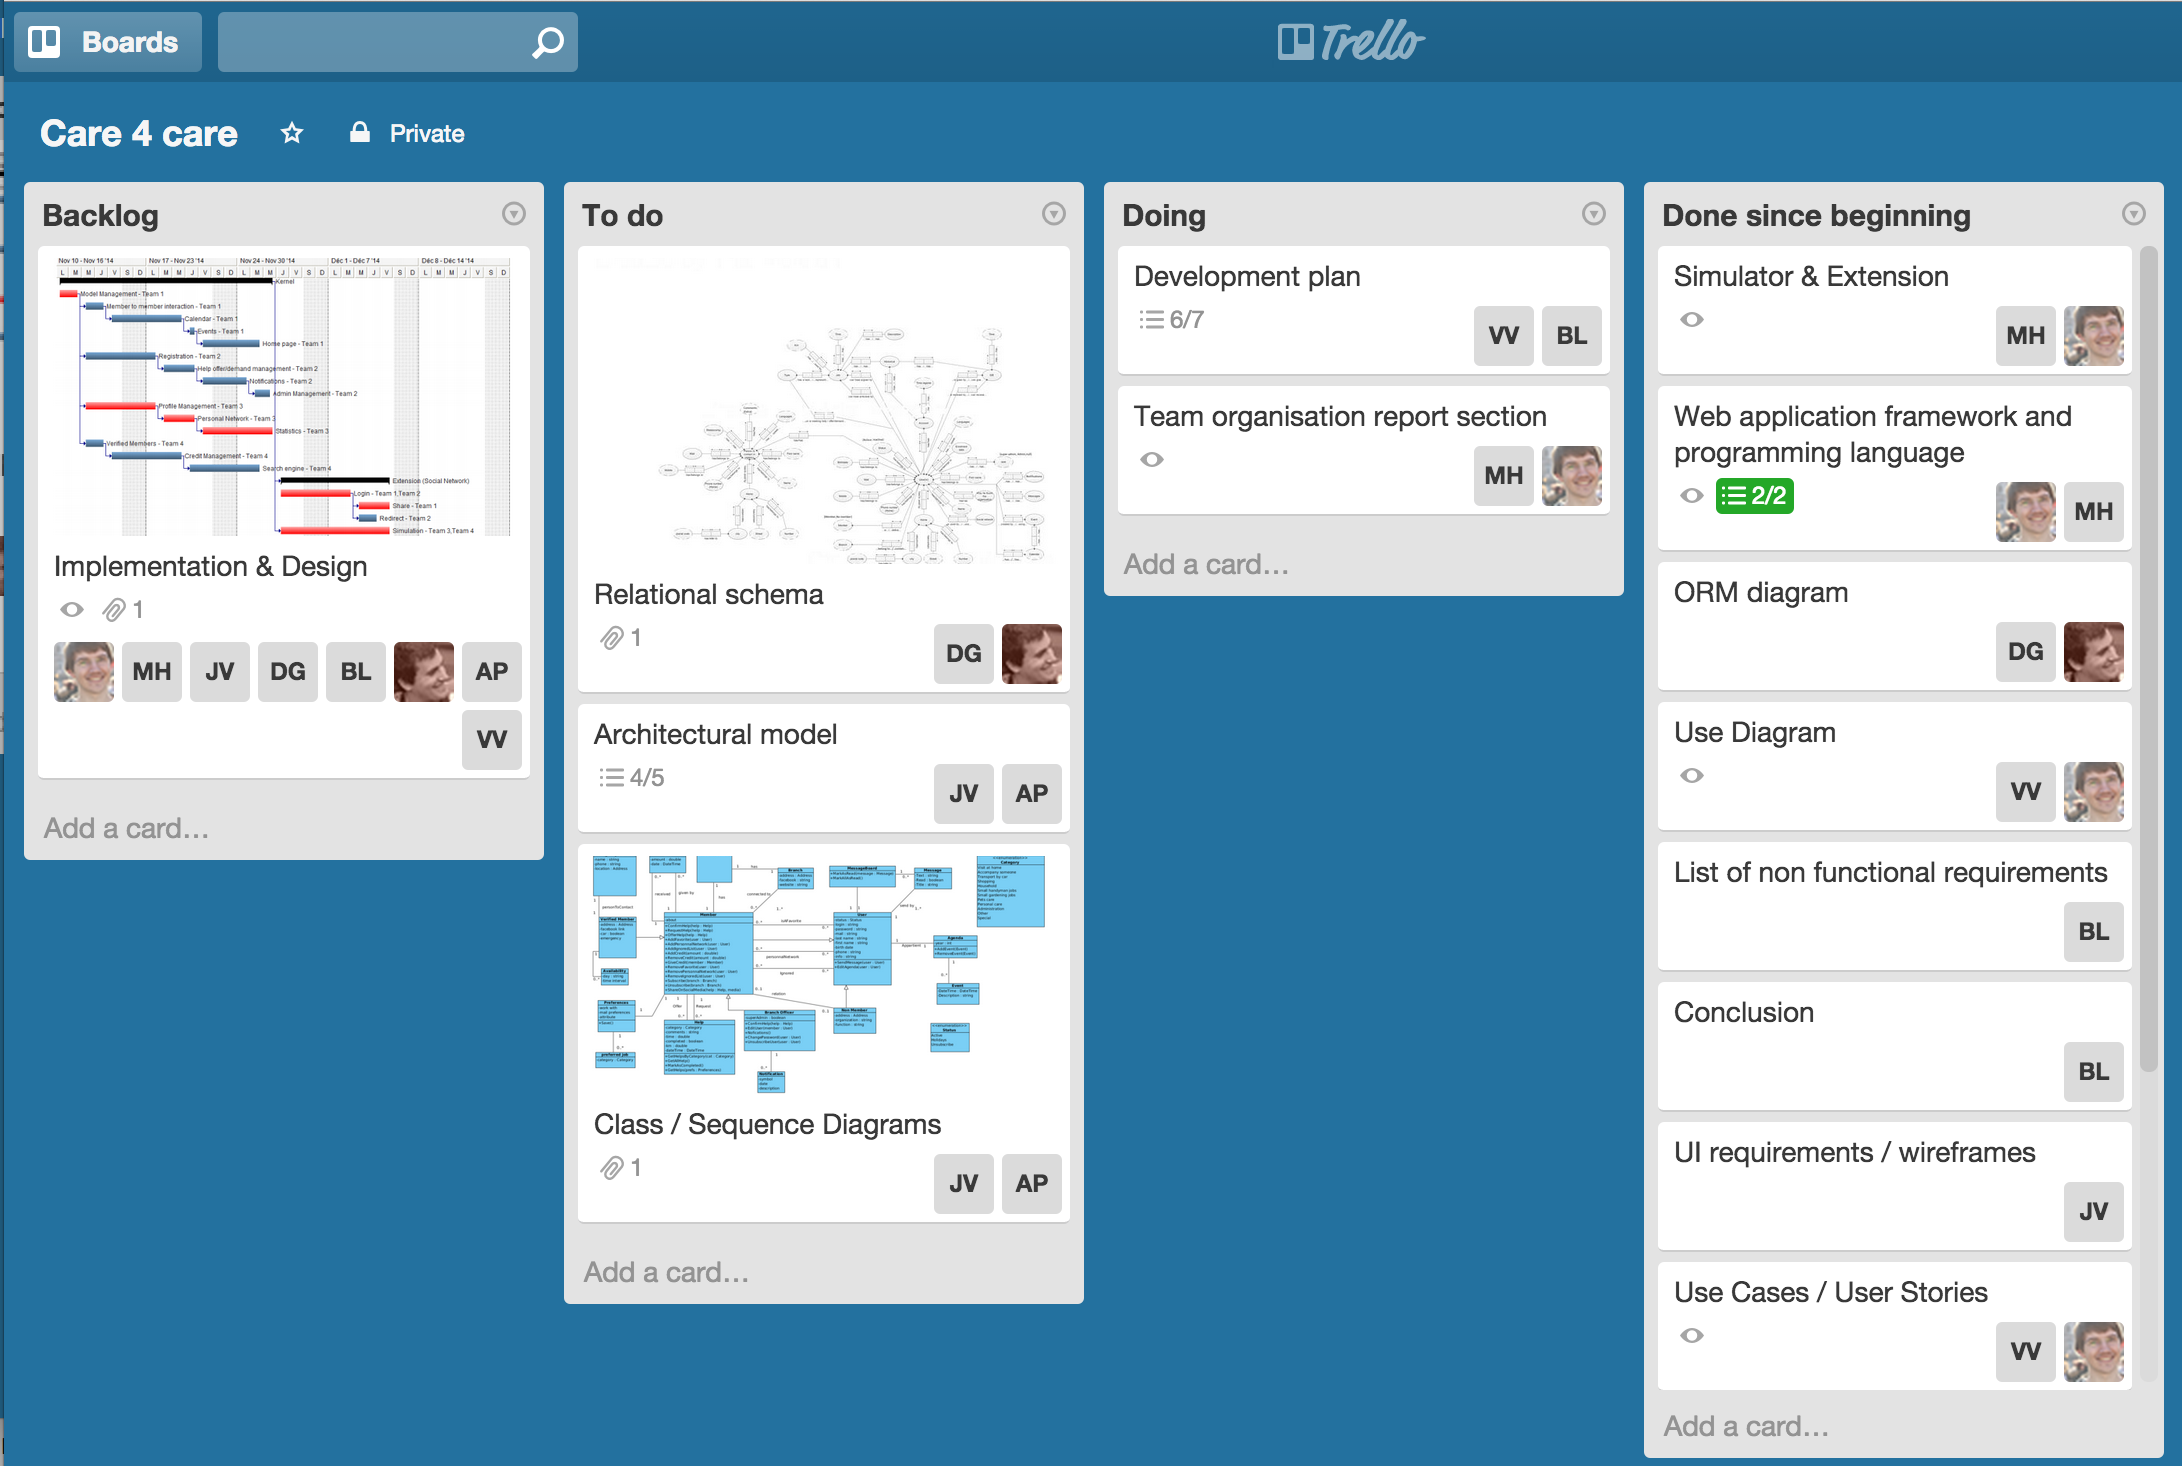
\includegraphics[width=\textwidth]{trello.png}
   \caption{\label{trello} Trello}
\end{figure}

Trello allows our team to organise the tasks scheduling.
We can create task and assign them to our members.
We are able to update each card and sort them by lists.
For the moment, as you can see on figure~\ref{trello}, we have four lists : \tit{Backlog}, \tit{To do}, \tit{Doing} and \tit{Done since beginning}.
This organisation is really helpful because we can see the progression in a glance.

\subsection{Github} 

\begin{figure}[!ht]
   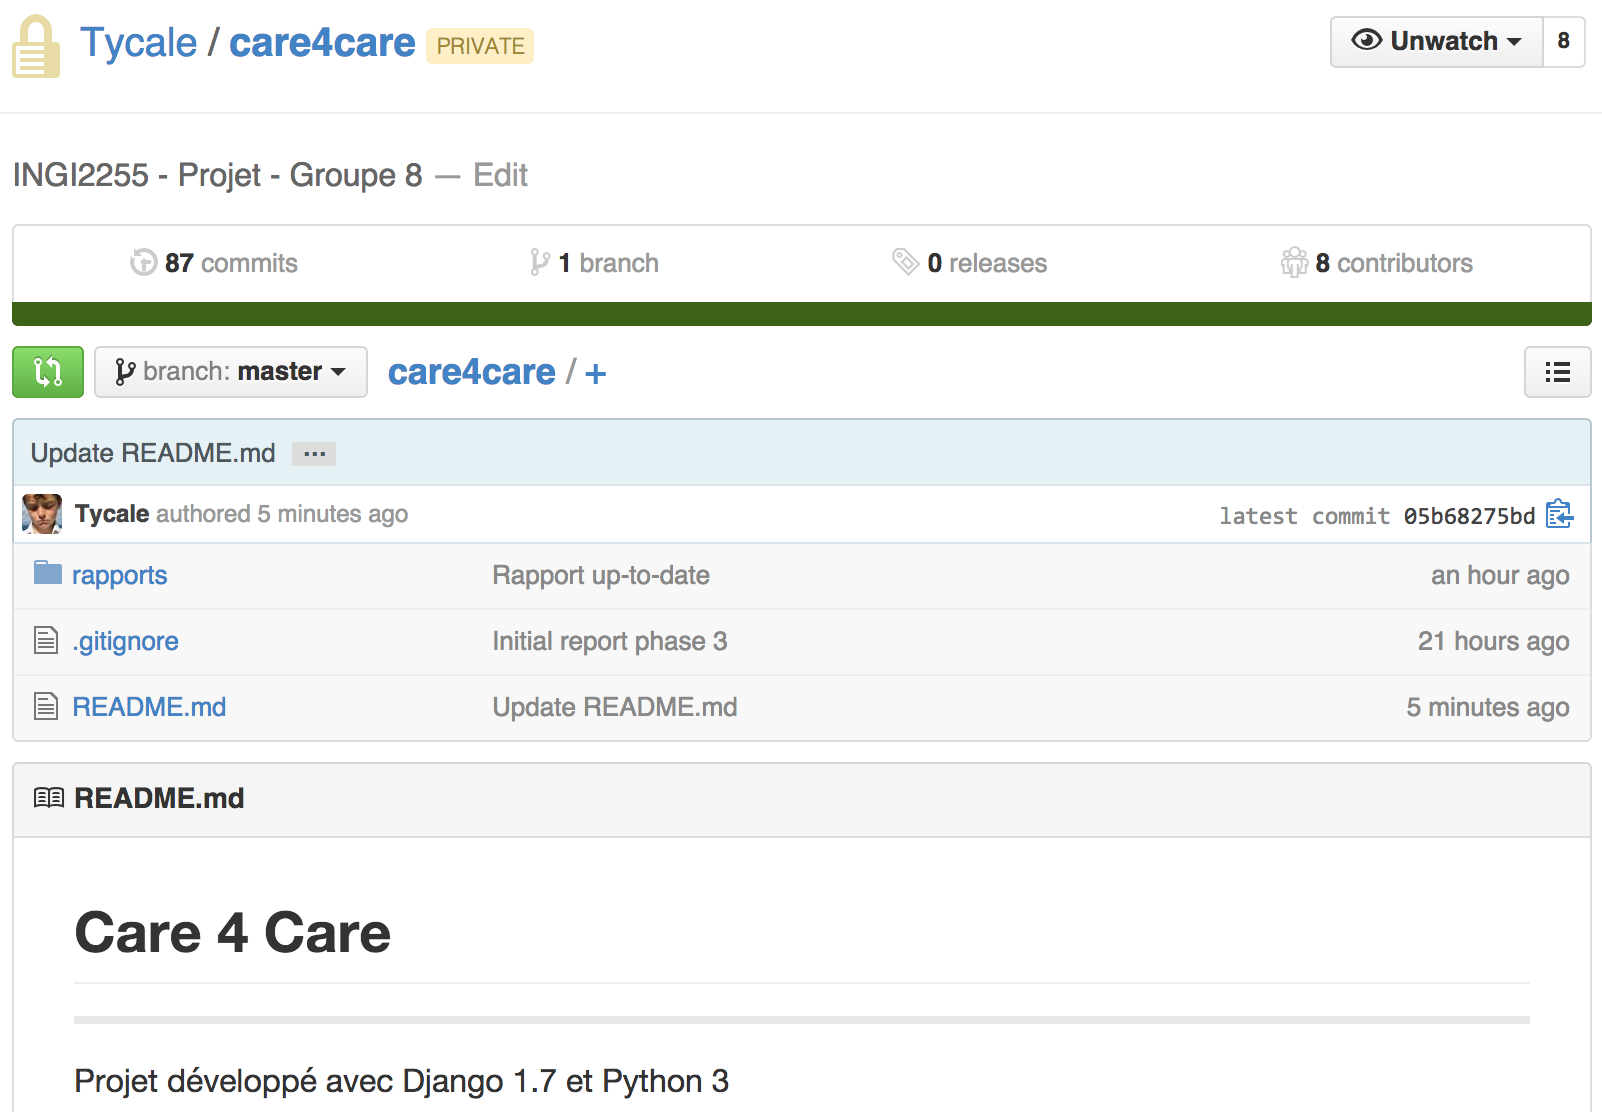
\includegraphics[width=\textwidth]{github.png}
   \caption{\label{github} github repository – care4care}
\end{figure}

Github is well-known in the developers community.
This platform permits us to synchronise the files and see the differences between versions.
We asked for a private repository thanks to the educational program.
The difference between two revisions is called a \enquote{commit}.
As shown in the figure~\ref{github}, you can see that we have 87 commits delivered by 8 contributors.


\end{document}
